% SSU Data Dash 2026: lab notebook. One entry per experiment, written as we go, so the
% report and the video can be written from it later. Not handed in.
%
% To log an experiment:
%   1. python run.py validate
%   2. python run.py report "what changed"   (adds row N to experiments.csv and writes
%      experiments/experiment_NN_results.tex and experiment_NN_error_by_price_range.png)
%   3. copy the entry template at the bottom of this file and fill it in.
%
% Compile from this folder, like report.tex (on Overleaf: upload the whole repository).
\documentclass[11pt]{article}
\usepackage[margin=2.2cm]{geometry}
\usepackage{graphicx,booktabs,hyperref}
\graphicspath{{experiments/}}
\setlength{\parskip}{4pt}

\title{SSU Data Dash 2026: lab notebook}
\date{}

\begin{document}
\maketitle

\section*{All experiments}
Validation scores of every logged run, in percent. Rows under different validation headings
are not comparable.

\begin{center}
\small
% Written by `python run.py report "what changed"`. Do not edit by hand: the log is report/experiments.csv.
\begin{tabular}{@{}rlp{6.5cm}cccc@{}}
\toprule
 & & & \multicolumn{2}{c}{Off-market} & \multicolumn{2}{c}{List-aware} \\
\cmidrule(lr){4-5}\cmidrule(l){6-7}
\# & Date & What changed & MdAPE \% & MAPE \% & MdAPE \% & MAPE \% \\
\midrule
\multicolumn{7}{@{}p{14cm}}{\textit{Validation: monthly walk-forward, 2025-12 to 2026-05: each month predicted from all sales before it}} \\
0 & 2026-10-23 & Starter baselines: 10 nearest earlier sales (off-market), list price (list-aware) & 20.84 & 27.43 & 7.26 & 8.09 \\
1 & 2026-10-23 & FeatureModel (gradient-boosted trees, starter features) on both tracks & 14.87 & 19.23 & 4.61 & 5.82 \\
\multicolumn{7}{@{}p{14cm}}{\textit{Validation: 4-month-ahead walk-forward, 2025-06 to 2026-05: 3 folds, each predicting 4 months from the sales before them}} \\
2 & 2026-10-23 & FeatureModel (gradient-boosted trees, starter features) on both tracks & 15.52 & 19.94 & 4.71 & 5.92 \\
3 & 2026-10-23 & Starter baselines under 4-month validation: 10 nearest earlier sales (off-market), list price (list-aware) & 20.94 & 27.84 & 7.17 & 8.00 \\
\bottomrule
\end{tabular}

\end{center}

% ---------------------------------------------------------------------------------------
\section*{Experiment 0: starter baselines}

\paragraph{What changed.}
Nothing: the starter code as given. Off-market predicts the median sold price of the 10 nearest
earlier sales of the same property type. List-aware predicts the list price.

\paragraph{Why.}
The reference point every later experiment is compared with.

\paragraph{Result.}

\begin{center}
\small
% Written by `python run.py report`. Do not edit by hand: rerun the command instead.
\begin{tabular}{lrccc}
\hline
Track & Homes & MdAPE \% (95\% CI) & MAPE \% (95\% CI) & Median signed error \% \\
\hline
off-market & 10,069 & 20.84 (20.40--21.36) & 27.43 (26.95--27.94) & +8.07 \\
list-aware & 10,069 & 7.26 (7.12--7.41) & 8.09 (7.98--8.20) & +5.68 \\
\hline
\end{tabular}

\end{center}

\begin{center}
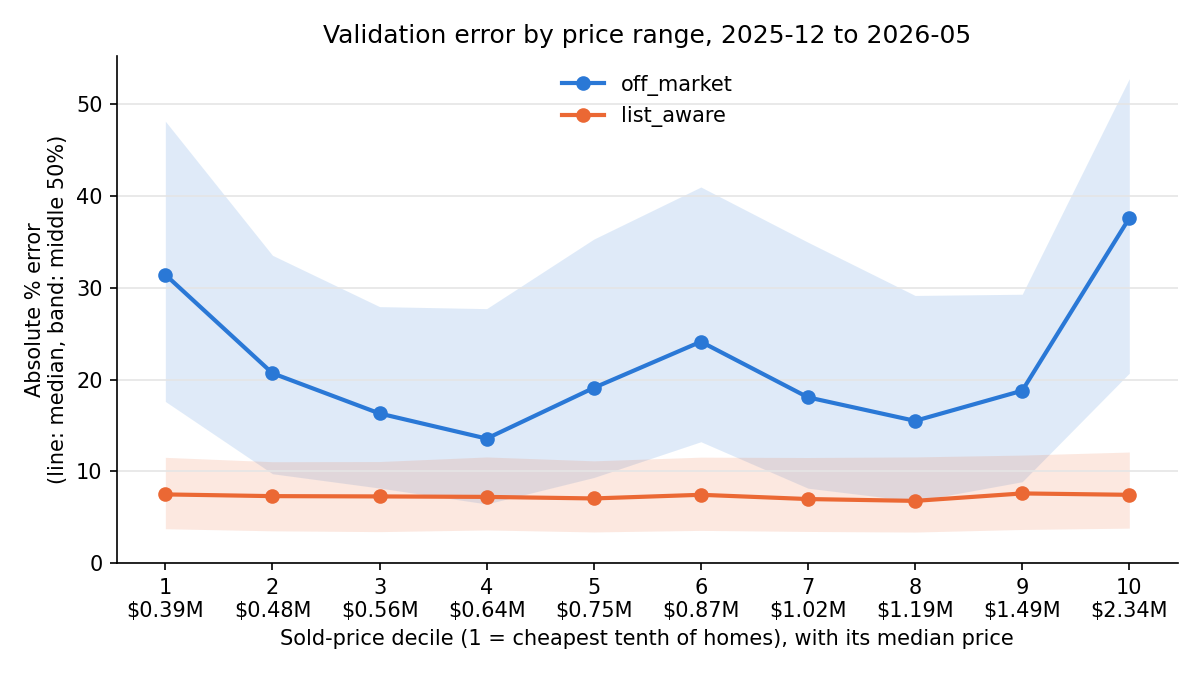
\includegraphics[width=0.8\linewidth]{experiment_00_error_by_price_range.png}
\end{center}

\paragraph{What we learned.}
\begin{itemize}
\item \textbf{Off-market misses the bar.} 20.84\% MdAPE is above the 17.7\% maximum error (the
  median sale of the same type in the same neighbourhood over the past 12 months), so as it stands
  it would earn no off-market accuracy points.
\item \textbf{Off-market predicts too high,} by 8.1\% at the median. The bias was largest in
  December 2025 (+14.4\%) and settled near +6 to +7\% by spring 2026. The comparable sales are
  not adjusted for how prices moved since they sold.
\item \textbf{Off-market pulls every home towards its neighbourhood's typical price.} It
  overprices the cheapest tenth of homes by 31\% and underprices the dearest tenth by 36\% (median
  signed error). The median of 10 neighbours ignores size, bedrooms and lot. Part of this pattern
  comes from grouping homes by their sold price, which exaggerates it for any model.
\item \textbf{Detached homes are hardest off-market:} 28.0\% MdAPE against 18.9\% for condo
  apartments. Their prices vary most with lot and size, which the baseline ignores.
\item \textbf{Homes sell below their list price.} The list price is 5.7\% too high at the
  median: 7.1\% for condo apartments and 0.5\% for semi-detached homes. Even a sold-to-list ratio
  per property type, learned from past sales, should beat the list-aware baseline.
\end{itemize}

\paragraph{Next.}
Switch on the gradient-boosted \texttt{FeatureModel} for both tracks, then make validation predict
up to four months ahead, as the hidden test does.

% ---------------------------------------------------------------------------------------
\section*{Experiment 1: gradient-boosted trees on the starter features}

\paragraph{What changed.}
\texttt{make\_model} now returns \texttt{FeatureModel} for both tracks: gradient-boosted trees
(scikit-learn's \texttt{HistGradientBoostingRegressor}, default settings) predicting log price from
the starter features. These are square feet, bedrooms, washrooms, parking, latitude, longitude,
months since January 2021 and property type, plus the list price for list-aware.

\paragraph{Why.}
Unlike the baselines, it can use each home's own size and features. The handout presents it as
the first model to switch on.

\paragraph{Result.}

\begin{center}
\small
% Written by `python run.py report`. Do not edit by hand: rerun the command instead.
\begin{tabular}{lrccc}
\hline
Track & Homes & MdAPE \% (95\% CI) & MAPE \% (95\% CI) & Median signed error \% \\
\hline
off-market & 10,069 & 14.87 (14.50--15.23) & 19.23 (18.92--19.57) & +1.02 \\
list-aware & 10,069 & 4.61 (4.50--4.71) & 5.82 (5.72--5.91) & +0.68 \\
\hline
\end{tabular}

\end{center}

\begin{center}
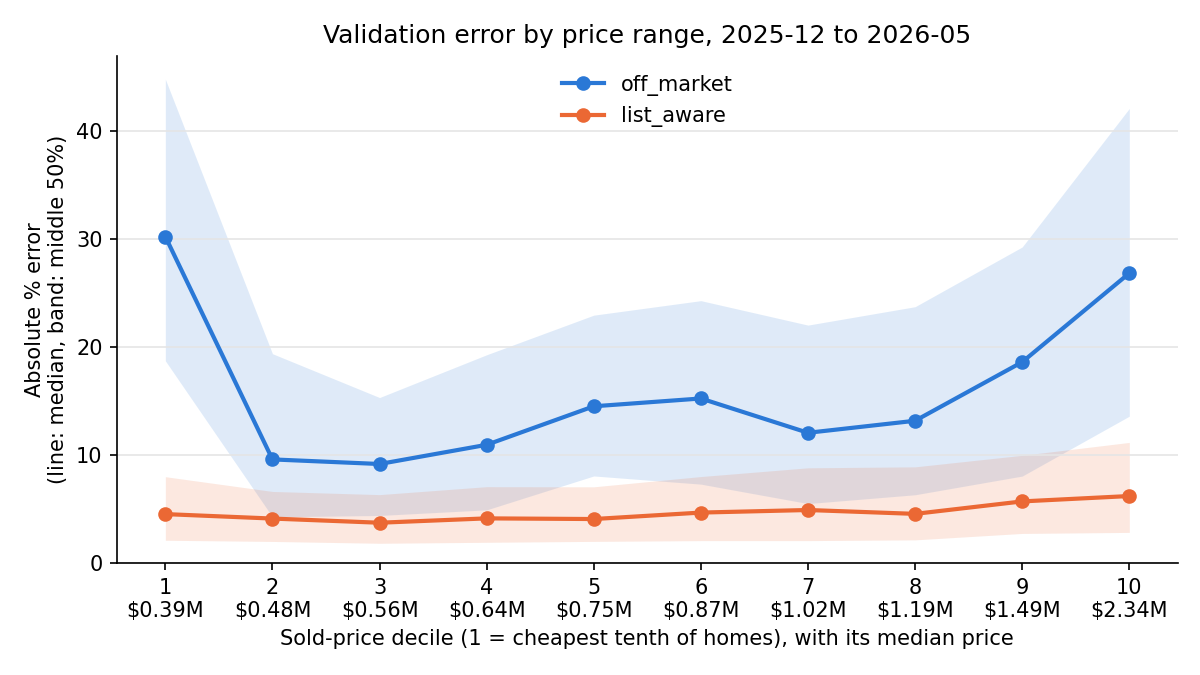
\includegraphics[width=0.8\linewidth]{experiment_01_error_by_price_range.png}
\end{center}

\paragraph{What we learned.}
\begin{itemize}
\item \textbf{A large gain on both tracks.} Off-market MdAPE fell from 20.84\% to 14.87\%, below
  the 17.7\% bar. List-aware fell from 7.26\% to 4.61\%: the model learns that homes sell below
  list, and by how much for each type.
\item \textbf{The overpricing is mostly gone:} median signed error +1.0\% off-market, +0.7\%
  list-aware.
\item \textbf{Off-market still squeezes prices towards the middle.} The cheapest tenth is
  overpriced by 30\% and the dearest tenth underpriced by 24\%. The features say little about
  what makes a home cheap or dear for its area: neighbourhood price level, lot size, condition.
\item \textbf{By type (off-market):} condo apartments 14.0\%, detached 17.3\%, co-op apartments
  26.0\% (only 48 homes). List-aware is weakest on semi-detached (6.1\%) and detached (5.9\%)
  homes.
\end{itemize}

\paragraph{Next.}
This validation predicts only one month ahead, but the hidden test predicts up to four. Fix that
before trusting any number.

% ---------------------------------------------------------------------------------------
\section*{Experiment 2: validation four months ahead, like the hidden test}

\paragraph{What changed.}
Validation only, not the model. Before, each month from December 2025 to May 2026 was predicted
from all sales before it, so always one month ahead. The hidden test trains on sales up to May
2026 and predicts homes sold June to September, one to four months ahead. Validation now does the
same in three folds: it trains on sales before June 2025, October 2025 and February 2026, and
predicts the four months after each, twelve months in all. The report gains a table of error by
months ahead.

\paragraph{Why.}
Validation should be a fair preview of the hidden test, since the judges compare the two (10
points for honesty). A one-month-ahead score overstates how well a model does four months out.

\paragraph{Result.}

\begin{center}
\small
% Written by `python run.py report`. Do not edit by hand: rerun the command instead.
\begin{tabular}{lrccc}
\hline
Track & Homes & MdAPE \% (95\% CI) & MAPE \% (95\% CI) & Median signed error \% \\
\hline
off-market & 22,238 & 15.52 (15.24--15.79) & 19.94 (19.71--20.16) & +3.02 \\
list-aware & 22,238 & 4.71 (4.63--4.79) & 5.92 (5.86--5.99) & +1.25 \\
\hline
\end{tabular}

\end{center}

\begin{center}
\small
\begin{tabular}{lcccc}
\toprule
Months ahead & 1 & 2 & 3 & 4 \\
\midrule
Off-market MdAPE \% & 14.4 & 15.8 & 15.9 & 16.1 \\
Off-market median signed error \% & +2.2 & +3.0 & +3.4 & +3.7 \\
List-aware MdAPE \% & 4.7 & 4.6 & 4.7 & 4.8 \\
\bottomrule
\end{tabular}
\end{center}

\paragraph{What we learned.}
\begin{itemize}
\item \textbf{The honest off-market error is 15.52\%, not 14.87\%,} and it rises from 14.4\% one
  month ahead to 16.1\% four months ahead. Part of the change from experiment 1 also comes from
  covering different months. The months-ahead table, all on the same homes, isolates the
  effect of the horizon.
\item \textbf{The model cannot follow the market past its last training month.} Trees hold the
  \texttt{months} feature at its last value. In the June to September 2025 fold the market was
  falling and off-market overpricing grew from +3.7\% in June to +9.8\% in August. In February to
  May 2026 it was slightly negative ($-0.6$ to $-2.2$\%). The bias follows whatever the market did
  after the cutoff.
\item \textbf{The fold most like the hidden test is the worst.} June to September 2025, the same
  season as the test, has off-market MdAPE from 14.7\% to 17.3\%.
\item \textbf{List-aware barely changes with the horizon} (4.6\% to 4.8\%): the list price already
  carries the current market.
\end{itemize}

\paragraph{Next.}
Starter baselines under this validation, to measure the gap fairly (experiment 3). Then a market
price index, so the model can project prices past May 2026.

% ---------------------------------------------------------------------------------------
\section*{Experiment 3: starter baselines under the four-month validation}

\paragraph{What changed.}
Nothing in the models: the starter baselines from experiment 0, rerun under the validation of
experiment 2. They were run by swapping them into \texttt{make\_model} for this one run, which
is why \texttt{experiments.csv} lists \texttt{models.py} as edited. The committed
\texttt{models.py} still uses \texttt{FeatureModel}.

\paragraph{Why.}
Scores from different validations cannot be compared. This gives the baseline row for the
report's results table, on the same homes as experiment 2.

\paragraph{Result.}

\begin{center}
\small
% Written by `python run.py report`. Do not edit by hand: rerun the command instead.
\begin{tabular}{lrccc}
\hline
Track & Homes & MdAPE \% (95\% CI) & MAPE \% (95\% CI) & Median signed error \% \\
\hline
off-market & 22,238 & 20.94 (20.63--21.28) & 27.84 (27.49--28.17) & +9.14 \\
list-aware & 22,238 & 7.17 (7.07--7.27) & 8.00 (7.92--8.06) & +5.75 \\
\hline
\end{tabular}

\end{center}

\begin{center}
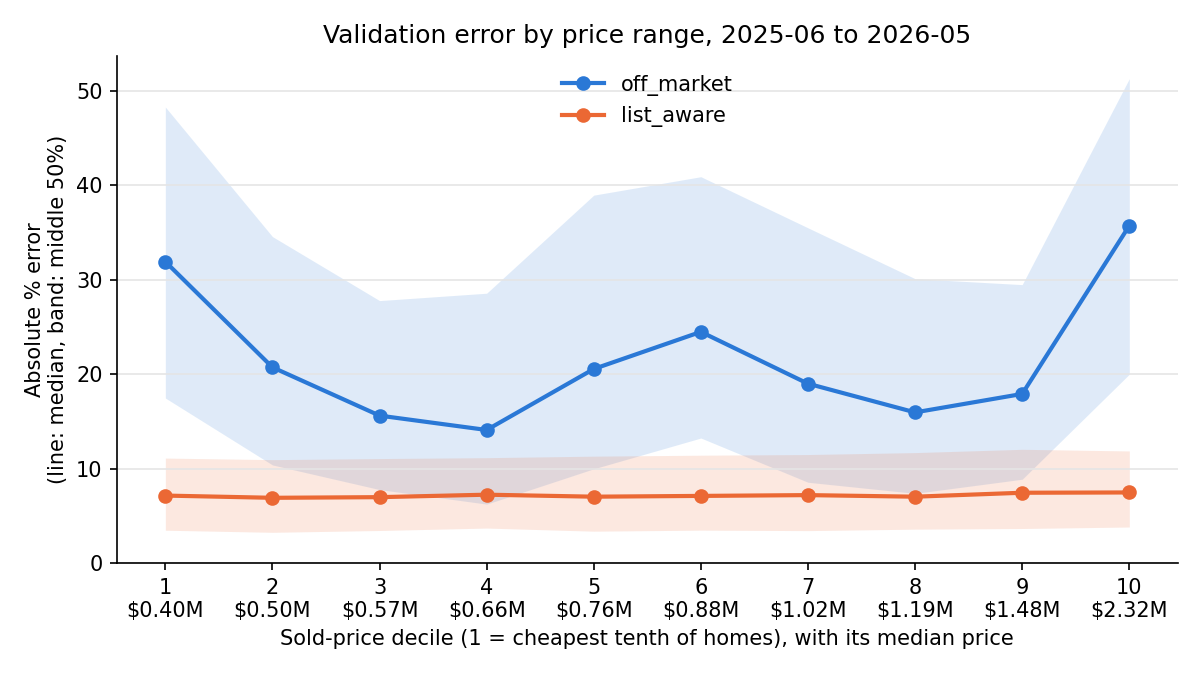
\includegraphics[width=0.8\linewidth]{experiment_03_error_by_price_range.png}
\end{center}

\paragraph{What we learned.}
\begin{itemize}
\item \textbf{On the same homes, \texttt{FeatureModel} beats the baselines by a wide margin.}
  Off-market MdAPE is 15.52\% against 20.94\%, and list-aware 4.71\% against 7.17\%.
\item \textbf{The baselines hardly change with the horizon} (off-market 20.5\% to 22.1\%, list
  price 7.1\% to 7.3\%). Their errors come mostly from ignoring the home's own features, not
  from how old the data is.
\item \textbf{The nearest-sales baseline overprices more the further ahead it predicts}
  (+7.9\% one month ahead, +9.3\% to +10.4\% after). Like \texttt{FeatureModel}, it does not
  adjust old sales for the market's movement.
\end{itemize}

\paragraph{Next.}
Measure the official bar (the median sale of the same type and neighbourhood over the past 12
months) under this validation, so we know our real margin above it. Then the market price index
and features that use past sales.

% ---------------------------------------------------------------------------------------
% Entry template: copy it above this line, replace NN with the experiment number.
%
% \section*{Experiment NN: short title}
% \paragraph{What changed.} The code change, in a sentence or two.
% \paragraph{Why.} The idea behind it: what we expected and why.
% \paragraph{Result.}
% \begin{center}\small\input{experiments/experiment_NN_results.tex}\end{center}
% \begin{center}\includegraphics[width=0.8\linewidth]{experiment_NN_error_by_price_range.png}\end{center}
% \paragraph{What we learned.} Did it work, where, and why we think so.
% \paragraph{Next.} What this suggests trying next.

\end{document}
